\documentclass[12pt,a4paper]{article}
\usepackage{fontspec}
\setmainfont{Times New Roman}[Path=C:/Windows/Fonts/,UprightFont=times.ttf,BoldFont=timesbd.ttf,ItalicFont=timesi.ttf,BoldItalicFont=timesbi.ttf]
\usepackage{amsmath,amssymb,amsfonts}
\usepackage[left=1.5cm,right=1.5cm,top=1.5cm,bottom=1.7cm,headheight=17pt]{geometry}
\usepackage{enumitem,array,graphicx,tikz,fancyhdr,needspace,booktabs}
\usetikzlibrary{patterns}

\pagestyle{fancy}
\fancyhf{}
\lhead{\small\textbf{ĐỀ CƯƠNG ÔN TẬP CHƯƠNG IV -- NGUYÊN HÀM VÀ TÍCH PHÂN}}
\rhead{\small\textit{Biên soạn: Dương Gia Bảo}}
\rfoot{\small Trang \thepage}
\renewcommand{\headrulewidth}{0.4pt}
\fancypagestyle{firstpage}{\fancyhead{}\renewcommand{\headrulewidth}{0pt}}

\setlength{\parindent}{0pt}
\setlength{\parskip}{3pt}
\setlength{\emergencystretch}{1em}

\setlist[enumerate,1]{label=\textbf{Câu \arabic*:},leftmargin=*,itemsep=6pt,topsep=4pt}

% Macro trắc nghiệm 4 phương án (giãn cách 8pt giữa hai hàng theo chuẩn nhánh)
\newcommand{\bonpa}[4]{\par\nobreak\smallskip\nobreak\noindent
\begin{tabular}{@{}p{0.48\linewidth}p{0.48\linewidth}@{}}
\textbf{A.} #1 & \textbf{B.} #2\\[8pt]
\textbf{C.} #3 & \textbf{D.} #4\end{tabular}}

% Macro khung ô li viết bài làm trực tiếp (kích thước rộng rãi 5mm x 5mm)
\newcommand{\khungOli}[1][5.2cm]{%
  \needspace{2.5cm}%
  \par\nobreak\vspace{4pt}\noindent
  \begin{tikzpicture}
    \pgfmathsetmacro{\gridw}{\linewidth - 1.5pt}
    \draw[step=0.5cm, line width=0.2pt, gray!32] (0,0) grid (\gridw pt, #1);
    \draw[line width=0.6pt, gray!60] (0,0) rectangle (\gridw pt, #1);
    \node[anchor=north east, font=\footnotesize\itshape\color{gray!60}, inner sep=4pt] at (\gridw pt, #1) {Bài làm của học sinh};
  \end{tikzpicture}
  \par\vspace{7pt}
}

\begin{document}
\thispagestyle{firstpage}

\noindent
\begin{minipage}[t]{0.36\textwidth}
    \centering
    {\fontsize{12}{14}\selectfont\textbf{ĐỀ CƯƠNG ÔN TẬP}}\\[4pt]
    \textit{Biên soạn: Dương Gia Bảo}\\[6pt]
    \setlength{\fboxrule}{0.8pt}
    \setlength{\fboxsep}{5pt}
    \fbox{\begin{minipage}{0.88\linewidth}
        \centering
        {\fontsize{12}{14}\selectfont\textbf{CHƯƠNG IV -- TOÁN 12}}
    \end{minipage}}
\end{minipage}\hfill
\begin{minipage}[t]{0.62\textwidth}
    \centering
    {\fontsize{13}{15}\selectfont\textbf{ĐỀ CƯƠNG ÔN TẬP CHƯƠNG IV}}\\[3pt]
    {\fontsize{12}{14}\selectfont\textbf{NGUYÊN HÀM VÀ TÍCH PHÂN}}\\[3pt]
    {\fontsize{11}{13}\selectfont\textit{(GDPT 2018 -- 20 Trắc nghiệm \& 30 Trả lời ngắn)}}
\end{minipage}

\par\vspace{4pt}
\hrule height 0.6pt
\vspace{4pt}
\noindent\textit{Họ và tên học sinh:}\dotfill\hspace{0.8cm}\textit{Lớp:}\makebox[3.2cm]{\dotfill}
\par\vspace{3pt}
\hrule height 0.6pt
\vspace{6pt}

%% ==============================================================
%% PHẦN I: TRẮC NGHIỆM (20 CÂU)
%% ==============================================================
\begin{center}
    {\fontsize{13}{15}\selectfont\textbf{PHẦN I. TRẮC NGHIỆM NHIỀU LỰA CHỌN (20 CÂU)}}
\end{center}

\begin{enumerate}
\item Cho hàm số $F(x)$ là một nguyên hàm của hàm số $f(x)$ trên khoảng $K$. Khẳng định nào sau đây đúng?
\bonpa{$f'(x) = F(x)$ với mọi $x \in K$}{$F'(x) = f(x)$ với mọi $x \in K$}{$F(x) = f(x) + C$ với mọi $x \in K$}{$F''(x) = f(x)$ với mọi $x \in K$}

\item Họ tất cả các nguyên hàm của hàm số $f(x) = 4x^3 + 3x^2 - 2$ là
\bonpa{$12x^2 + 6x + C$}{$x^4 + x^3 - 2 + C$}{$\dfrac{x^4}{4} + \dfrac{x^3}{3} - 2x + C$}{$x^4 + x^3 - 2x + C$}

\item Trên khoảng $(0; +\infty)$, họ nguyên hàm của hàm số $f(x) = \dfrac{3}{x} + \sqrt{x}$ là
\bonpa{$3\ln x + \dfrac{2}{3}x\sqrt{x} + C$}{$3\ln x + \dfrac{1}{2\sqrt{x}} + C$}{$-\dfrac{3}{x^2} + \dfrac{2}{3}x\sqrt{x} + C$}{$\dfrac{3}{2}\ln x + \dfrac{2}{3}\sqrt{x^3} + C$}

\item Tìm họ nguyên hàm của hàm số $f(x) = \dfrac{1}{\sin^2 x} - 3\cos x$ trên mỗi khoảng xác định của $f(x)$.
\bonpa{$\cot x - 3\sin x + C$}{$-\cot x + 3\sin x + C$}{$-\cot x - 3\sin x + C$}{$\tan x - 3\sin x + C$}

\item Họ nguyên hàm của hàm số $f(x) = 2^x + 3\mathrm{e}^x$ là
\bonpa{$\dfrac{2^x}{\ln 2} + 3\mathrm{e}^x + C$}{$2^x \ln 2 + 3\mathrm{e}^x + C$}{$\dfrac{2^{x+1}}{x+1} + 3\mathrm{e}^x + C$}{$\dfrac{2^x}{\ln 2} + \mathrm{e}^{3x} + C$}

\item Cho hàm số $f(x) = 6x^2 - 4x + 1$. Biết $F(x)$ là một nguyên hàm của $f(x)$ thỏa mãn $F(0) = 3$. Giá trị của $F(2)$ bằng
\bonpa{$9$}{$10$}{$11$}{$13$}

\item Một chất điểm bắt đầu chuyển động từ trạng thái đứng yên ($v(0) = 0$) với gia tốc tại thời điểm $t$ giây ($t \ge 0$) được cho bởi $a(t) = 4t + 2$ ($\text{m/s}^2$). Vận tốc của chất điểm tại thời điểm $t = 3$ giây là
\bonpa{$14\text{ m/s}$}{$24\text{ m/s}$}{$18\text{ m/s}$}{$20\text{ m/s}$}

\item Cho hàm số $f(x)$ liên tục trên $[a; b]$ và $F(x)$ là một nguyên hàm của $f(x)$ trên $[a; b]$. Nếu $F(a) = 7$ và $F(b) = -3$ thì giá trị của tích phân $\int_a^b f(x)\,\mathrm{d}x$ bằng
\bonpa{$4$}{$10$}{$-10$}{$-4$}

\item Cho hàm số $f(x)$ liên tục trên $\mathbb{R}$ thỏa mãn $\int_{-1}^5 f(x)\,\mathrm{d}x = 12$ và $\int_{-1}^2 f(x)\,\mathrm{d}x = 5$. Giá trị của tích phân $\int_2^5 f(x)\,\mathrm{d}x$ bằng
\bonpa{$7$}{$17$}{$-7$}{$60$}

\item Cho $\int_1^3 f(x)\,\mathrm{d}x = 4$ và $\int_1^3 g(x)\,\mathrm{d}x = -1$. Giá trị của tích phân $I = \int_1^3 [5f(x) + 3g(x)]\,\mathrm{d}x$ bằng
\bonpa{$23$}{$19$}{$16$}{$17$}

\item Giá trị của tích phân $I = \int_0^1 (4x^3 + 3\mathrm{e}^x)\,\mathrm{d}x$ bằng
\bonpa{$3\mathrm{e} - 1$}{$3\mathrm{e} - 2$}{$3\mathrm{e} + 1$}{$3\mathrm{e} - 3$}

\item Giá trị của tích phân $I = \int_0^{\frac{\pi}{4}} (2\cos 2x + 1)\,\mathrm{d}x$ bằng
\bonpa{$\dfrac{\pi}{4}$}{$2 + \dfrac{\pi}{4}$}{$1 + \dfrac{\pi}{4}$}{$-1 + \dfrac{\pi}{4}$}

\item Giá trị của tích phân $I = \int_{-1}^2 |2x|\,\mathrm{d}x$ bằng
\bonpa{$5$}{$3$}{$4$}{$6$}

\item Giá trị của tích phân $I = \int_1^2 \dfrac{2}{x}\,\mathrm{d}x$ bằng
\bonpa{$\ln 2$}{$\ln 4$}{$\dfrac{3}{2}$}{$2\ln 4$}

\item Diện tích $S$ của hình phẳng giới hạn bởi hai đồ thị hàm số liên tục $y = f(x)$, $y = g(x)$ và hai đường thẳng $x = a$, $x = b$ ($a < b$) được tính theo công thức nào sau đây?
\bonpa{$S = \pi\int_a^b |f(x) - g(x)|\,\mathrm{d}x$}{$S = \int_a^b [f(x) - g(x)]\,\mathrm{d}x$}{$S = \pi\int_a^b [f^2(x) - g^2(x)]\,\mathrm{d}x$}{$S = \int_a^b |f(x) - g(x)|\,\mathrm{d}x$}

\item Diện tích hình phẳng giới hạn bởi parabol $y = 4 - x^2$ và trục hoành $Ox$ bằng
\bonpa{$\dfrac{16}{3}$}{$\dfrac{32\pi}{3}$}{$\dfrac{32}{3}$}{$\dfrac{64}{3}$}

\item Diện tích hình phẳng giới hạn bởi hai đồ thị hàm số $y = x^2 - 1$ và $y = 1 - x^2$ bằng
\bonpa{$\dfrac{4}{3}$}{$\dfrac{8}{3}$}{$\dfrac{16}{3}$}{$2$}

\item Cho một vật thể nằm giữa hai mặt phẳng $x = 0$ và $x = 2$. Biết thiết diện của vật thể bị cắt bởi mặt phẳng vuông góc với trục $Ox$ tại điểm có hoành độ $x$ ($0 \le x \le 2$) là một hình vuông có độ dài cạnh bằng $\sqrt{3x + 1}$. Thể tích $V$ của vật thể đó bằng
\bonpa{$8$}{$8\pi$}{$7$}{$10$}

\item Thể tích $V$ của khối tròn xoay thu được khi quay hình phẳng giới hạn bởi đường cong $y = \mathrm{e}^x$, trục hoành $Ox$ và hai đường thẳng $x = 0$, $x = 1$ quanh trục $Ox$ là
\bonpa{$\dfrac{\mathrm{e}^2 - 1}{2}$}{$\pi(\mathrm{e}^2 - 1)$}{$\dfrac{\pi(\mathrm{e} - 1)}{2}$}{$\dfrac{\pi(\mathrm{e}^2 - 1)}{2}$}

\item Một máy bơm nước vào bể với lưu lượng tại thời điểm $t$ giây ($t \ge 0$) là $Q(t) = 3t^2 + 2t$ (lít/giây). Lượng nước bơm được vào bể từ giây thứ $1$ đến giây thứ $4$ là
\bonpa{$80$ lít}{$72$ lít}{$78$ lít}{$64$ lít}
\end{enumerate}

\newpage
%% ==============================================================
%% PHẦN II: TRẢ LỜI NGẮN (30 CÂU)
%% ==============================================================
\begin{center}
    {\fontsize{13}{15}\selectfont\textbf{PHẦN II. TRẢ LỜI NGẮN KÈM Ô LI LÀM BÀI (30 CÂU)}}
\end{center}

\subsubsection*{Mạch 1. Bài 11: Nguyên hàm và ứng dụng thực tế (Câu 21 -- 30)}

\begin{enumerate}[start=21]
\needspace{7.6cm}
\item Cho hàm số $f(x) = 3x^2 - 8x + 5$. Biết $F(x)$ là một nguyên hàm của $f(x)$ thỏa mãn $F(1) = 6$. Tính giá trị của $F(4)$.
\khungOli[5.0cm]

\needspace{7.6cm}
\item Cho hàm số $f(x) = 2x + \dfrac{6}{\sqrt{x}}$ xác định trên $(0; +\infty)$. Biết $F(x)$ là một nguyên hàm của $f(x)$ thỏa mãn $F(1) = 10$. Tính giá trị của $F(9)$.
\khungOli[5.0cm]

\needspace{7.6cm}
\item Cho hàm số $f(x) = \dfrac{2x^2 - x + 3}{x}$ trên khoảng $(0; +\infty)$. Biết $F(x)$ là một nguyên hàm của $f(x)$ thỏa mãn $F(1) = 4$ và $F(\mathrm{e}) = \mathrm{e}^2 - \mathrm{e} + c$. Tìm giá trị của hằng số $c$.
\khungOli[5.0cm]

\needspace{7.6cm}
\item Cho hàm số $f(x) = 4\sin x + 2\cos x$. Biết $F(x)$ là một nguyên hàm của $f(x)$ thỏa mãn $F(0) = 3$. Tính giá trị của $F(\pi)$.
\khungOli[5.0cm]

\needspace{7.8cm}
\item Gọi $F(x)$ là một nguyên hàm của hàm số $f(x) = \tan^2 x$ trên khoảng $\left(-\dfrac{\pi}{2}; \dfrac{\pi}{2}\right)$ thỏa mãn $F(0) = 2$. Biết rằng $F\!\left(\dfrac{\pi}{4}\right) = a - \dfrac{\pi}{b}$ với $a, b \in \mathbb{Z}^+$. Tính giá trị của $a + b$.
\khungOli[5.2cm]

\needspace{7.6cm}
\item Gọi $F(x)$ là một nguyên hàm của hàm số $f(x) = \mathrm{e}^x(2 + \mathrm{e}^{-x})$ thỏa mãn $F(0) = 5$. Biết rằng $F(\ln 3) = a + \ln b$ với $a, b \in \mathbb{Z}^+$. Tính giá trị của $a + b$.
\khungOli[5.0cm]

\needspace{7.6cm}
\item Một đường cong $(C): y = f(x)$ có hệ số góc của tiếp tuyến tại mỗi điểm có hoành độ $x$ bằng $f'(x) = 3x^2 - 4x + 2$. Biết đồ thị hàm số đi qua điểm $M(2; 11)$, hãy tính giá trị của $f(3)$.
\khungOli[5.0cm]

\needspace{7.8cm}
\item Một cây xanh được trồng với chiều cao ban đầu lúc mới trồng ($t = 0$) là $45\text{ cm}$. Trong $10$ năm đầu, tốc độ tăng trưởng chiều cao của cây (tính theo $\text{cm/năm}$) được mô hình hóa bởi $h'(t) = 1{,}5t + 20$, với $t$ là số năm kể từ lúc trồng. Hỏi sau $6$ năm, cây cao bao nhiêu $\text{cm}$?
\khungOli[5.0cm]

\needspace{8.0cm}
\item Tại một xưởng sản xuất, hàm chi phí biên khi sản xuất $x$ đơn vị sản phẩm được cho bởi $C'(x) = 0{,}06x^2 - 1{,}2x + 15$ (triệu đồng/sản phẩm), biết chi phí cố định ban đầu $C(0) = 80$ triệu đồng. Tính tổng chi phí (triệu đồng) để sản xuất $20$ đơn vị sản phẩm đầu tiên.
\khungOli[5.2cm]

\needspace{8.0cm}
\item Một vật được ném thẳng đứng lên cao từ độ cao $25\text{ m}$ so với mặt đất với vận tốc ban đầu $v_0 = 20\text{ m/s}$. Biết gia tốc của vật không đổi bằng $a(t) = -10\text{ m/s}^2$. Tính độ cao lớn nhất (đơn vị: mét) mà vật đạt được so với mặt đất.
\khungOli[5.2cm]

\needspace{9.0cm}
\subsubsection*{Mạch 2. Bài 12: Tích phân và ứng dụng thực tế (Câu 31 -- 40)}

\needspace{7.8cm}
\item Cho hai hàm số $f(x), g(x)$ liên tục trên $[0; 4]$ thỏa mãn $\int_0^4 [2f(x) + g(x)]\,\mathrm{d}x = 19$ và $\int_0^4 [f(x) - g(x)]\,\mathrm{d}x = 2$. Tính giá trị của tích phân $I = \int_0^4 [3f(x) + 4g(x)]\,\mathrm{d}x$.
\khungOli[5.2cm]

\needspace{7.6cm}
\item Biết tích phân $\int_0^2 \dfrac{2x + 5}{x + 1}\,\mathrm{d}x = a + b\ln 3$ với $a, b \in \mathbb{Z}$. Tính giá trị của biểu thức $P = a^2 + b^2$.
\khungOli[5.0cm]

\needspace{7.6cm}
\item Tính giá trị của tích phân $I = \int_1^4 \dfrac{x^2 + 3\sqrt{x}}{\sqrt{x}}\,\mathrm{d}x$ (viết kết quả dưới dạng số thập phân).
\khungOli[5.0cm]

\needspace{7.6cm}
\item Biết tích phân $\int_0^{\frac{\pi}{2}} (2\sin x + 3\cos x - 1)\,\mathrm{d}x = a - \dfrac{\pi}{b}$ với $a, b \in \mathbb{Z}^+$. Tính giá trị của $a + b$.
\khungOli[5.0cm]

\needspace{8.2cm}
\item Tính tích phân $I = \int_0^3 |x^2 - 2x|\,\mathrm{d}x$. Biết kết quả viết được dưới dạng phân số tối giản $\dfrac{a}{b}$ với $a, b \in \mathbb{Z}^+$, hãy tính giá trị của $a + b$.
\khungOli[5.5cm]

\needspace{8.0cm}
\item Cho hàm số $f(x) = \begin{cases} 4x - 1 & \text{khi } x \ge 2 \\ x^2 + 3 & \text{khi } x < 2 \end{cases}$. Tính giá trị của tích phân $I = \int_{-1}^4 f(x)\,\mathrm{d}x$.
\khungOli[5.2cm]

\needspace{7.6cm}
\item Tìm số thực dương $m$ thỏa mãn đẳng thức tích phân $\int_0^m (3x^2 - 4x + 4)\,\mathrm{d}x = 8$.
\khungOli[5.0cm]

\needspace{8.4cm}
\item Một chất điểm chuyển động thẳng với vận tốc tại thời điểm $t$ giây ($0 \le t \le 4$) được cho bởi $v(t) = t^2 - 4t + 3$ ($\text{m/s}$). Tính tổng quãng đường (đơn vị: mét) chất điểm đi được trong $4$ giây đầu tiên.
\khungOli[5.8cm]

\needspace{12.2cm}
\item Một xe ô tô chuyển động trên đường thẳng trong $30$ giây đầu tiên có đồ thị vận tốc $v(t)$ ($\text{m/s}$) theo thời gian $t$ (giây) là đường gấp khúc $OABC$ như hình vẽ bên dưới. Tính quãng đường (đơn vị: mét) mà ô tô đi được trong $30$ giây đó (viết kết quả dưới dạng số thập phân).
\begin{center}
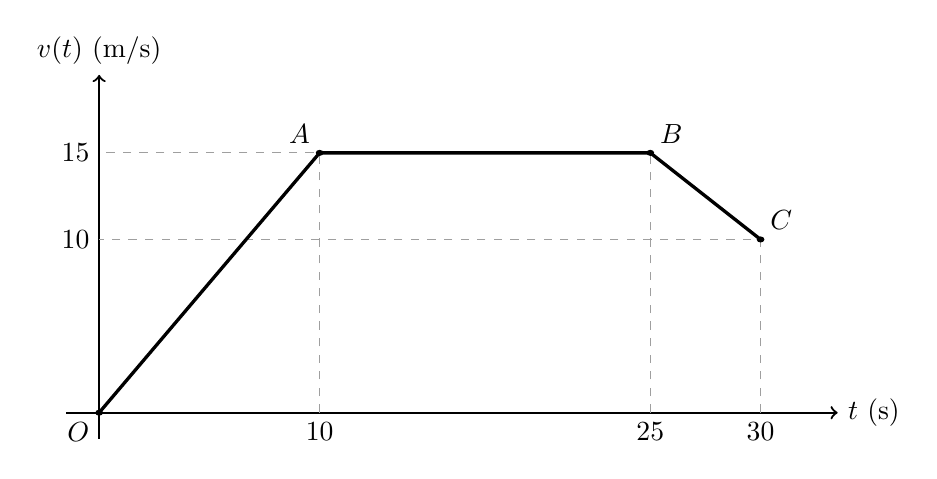
\begin{tikzpicture}[xscale=0.28, yscale=0.22]
  \draw[->, line width=0.8pt] (-1.5,0) -- (33.5,0) node[right] {$t\text{ (s)}$};
  \draw[->, line width=0.8pt] (0,-1.5) -- (0,19.5) node[above] {$v(t)\text{ (m/s)}$};
  \draw[dashed, gray!75] (10,0) -- (10,15) -- (0,15);
  \draw[dashed, gray!75] (25,0) -- (25,15);
  \draw[dashed, gray!75] (30,0) -- (30,10) -- (0,10);
  \draw[line width=1.2pt] (0,0) -- (10,15) -- (25,15) -- (30,10);
  \fill (0,0) circle (5pt) node[below left] {$O$};
  \fill (10,15) circle (5pt) node[above left] {$A$};
  \fill (25,15) circle (5pt) node[above right] {$B$};
  \fill (30,10) circle (5pt) node[above right] {$C$};
  \node[below] at (10,0) {$10$};
  \node[below] at (25,0) {$25$};
  \node[below] at (30,0) {$30$};
  \node[left] at (0,10) {$10$};
  \node[left] at (0,15) {$15$};
\end{tikzpicture}
\end{center}
\khungOli[5.0cm]

\needspace{7.8cm}
\item Công suất tiêu thụ điện của một trạm bơm nước nông nghiệp tại thời điểm $t$ giờ ($0 \le t \le 6$) được mô tả bởi hàm số $P(t) = 12 + 6t - 0{,}75t^2$ ($\text{kW}$). Tính tổng điện năng tiêu thụ $E = \int_0^6 P(t)\,\mathrm{d}t$ (đơn vị: $\text{kWh}$) của trạm bơm trong $6$ giờ hoạt động liên tục đó.
\khungOli[5.0cm]

\needspace{9.0cm}
\subsubsection*{Mạch 3. Bài 13: Ứng dụng hình học của tích phân \& Bài tập cuối chương (Câu 41 -- 50)}

\needspace{7.6cm}
\item Tính diện tích hình phẳng giới hạn bởi đường cong $y = x^3 - 4x$ và trục hoành $Ox$.
\khungOli[5.2cm]

\needspace{7.6cm}
\item Tính diện tích hình phẳng giới hạn bởi parabol $y = x^2 - 4x + 5$ và đường thẳng $y = -x + 5$ (viết kết quả dưới dạng số thập phân).
\khungOli[5.0cm]

\needspace{12.2cm}
\item Cho hàm số $y = f(x)$ liên tục trên $\mathbb{R}$ có đồ thị cắt trục hoành tại ba điểm có hoành độ lần lượt là $-2; 1; 4$ như hình vẽ. Biết diện tích hai phần hình phẳng gạch chéo lần lượt là $S_1 = 11$ và $S_2 = 6$. Tính giá trị của tích phân $I = \int_{-2}^4 [2f(x) + 3]\,\mathrm{d}x$.
\begin{center}
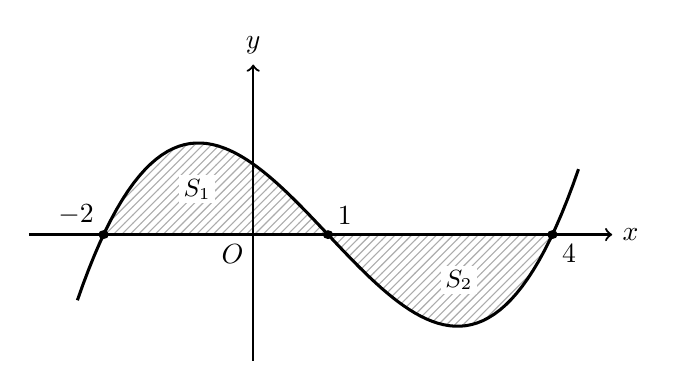
\begin{tikzpicture}[xscale=0.95, yscale=0.8]
  % Đồ thị mô phỏng cắt tại -2, 1, 4: y = +0.14*(x+2)*(x-1)*(x-4) -> y > 0 tren (-2,1), y < 0 tren (1,4)
  \fill[pattern=north east lines, pattern color=gray!65]
    plot[domain=-2:1, samples=60] (\x, {0.14*(\x+2)*(\x-1)*(\x-4)}) -- (1,0) -- (-2,0) -- cycle;
  \fill[pattern=north east lines, pattern color=gray!65]
    plot[domain=1:4, samples=60] (\x, {0.14*(\x+2)*(\x-1)*(\x-4)}) -- (4,0) -- (1,0) -- cycle;
  \draw[->, line width=0.8pt] (-3.0,0) -- (4.8,0) node[right] {$x$};
  \draw[->, line width=0.8pt] (0,-2.0) -- (0,2.7) node[above] {$y$};
  \draw[line width=1.1pt] plot[domain=-2.35:4.35, samples=90] (\x, {0.14*(\x+2)*(\x-1)*(\x-4)});
  \fill (-2,0) circle (2pt) node[above left] {$-2$};
  \fill (1,0) circle (2pt) node[above right] {$1$};
  \fill (4,0) circle (2pt) node[below right] {$4$};
  \node[below left] at (0,0) {$O$};
  \node[fill=white, inner sep=1.5pt, font=\small] at (-0.75, 0.72) {$S_1$};
  \node[fill=white, inner sep=1.5pt, font=\small] at (2.75, -0.72) {$S_2$};
\end{tikzpicture}
\end{center}
\khungOli[5.0cm]

\needspace{12.5cm}
\item Trên một viên gạch hoa hình vuông $OABC$ cạnh $6\text{ dm}$ đặt trong hệ trục tọa độ $Oxy$ như hình vẽ bên dưới ($O(0;0), A(6;0), B(6;6), C(0;6)$, đơn vị trên mỗi trục là $\text{dm}$), người ta thiết kế một cánh hoa (phần gạch chéo) giới hạn bởi hai đường parabol $(P_1): y = \dfrac{1}{6}x^2$ và $(P_2): y = -\dfrac{1}{6}x^2 + 2x$. Tính diện tích của cánh hoa đó (đơn vị: $\text{dm}^2$).
\begin{center}
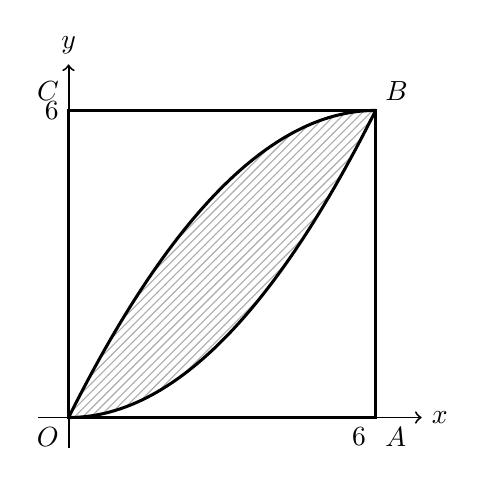
\begin{tikzpicture}[scale=0.65]
  % Hình vuông [0,6] x [0,6]
  \fill[pattern=north east lines, pattern color=gray!65]
    plot[domain=0:6, samples=60] (\x, {-\x*\x/6 + 2*\x}) --
    plot[domain=6:0, samples=60] (\x, {\x*\x/6}) -- cycle;
  \draw[line width=0.9pt] (0,0) rectangle (6,6);
  \draw[->, line width=0.7pt] (-0.6,0) -- (6.9,0) node[right] {$x$};
  \draw[->, line width=0.7pt] (0,-0.6) -- (0,6.9) node[above] {$y$};
  \draw[line width=1.1pt] plot[domain=0:6, samples=60] (\x, {\x*\x/6});
  \draw[line width=1.1pt] plot[domain=0:6, samples=60] (\x, {-\x*\x/6 + 2*\x});
  \node[below left] at (0,0) {$O$};
  \node[below left] at (6,0) {$6$};
  \node[below right] at (6,0) {$A$};
  \node[above right] at (6,6) {$B$};
  \node[left] at (0,6) {$6$};
  \node[above left] at (0,6) {$C$};
\end{tikzpicture}
\end{center}
\khungOli[5.0cm]

\needspace{8.5cm}
\item Mặt cắt ngang của một đường hầm giao thông có dạng một hình parabol với chiều rộng mặt đường dưới chân hầm là $12\text{ m}$ và chiều cao lớn nhất ở chính giữa hầm là $9\text{ m}$. Người ta cần lắp đặt lưới chắn bảo vệ toàn bộ phần diện tích mặt cắt ngang của cửa hầm với đơn giá $0{,}5$ triệu đồng/$\text{m}^2$. Tính tổng chi phí làm lưới chắn (đơn vị: triệu đồng).
\khungOli[5.5cm]

\needspace{8.2cm}
\item Một vật thể giới hạn bởi hai mặt phẳng vuông góc với trục $Ox$ tại $x = 1$ và $x = 4$. Cắt vật thể bởi mặt phẳng vuông góc với trục $Ox$ tại điểm có hoành độ $x$ ($1 \le x \le 4$), thiết diện thu được là một tam giác vuông cân có độ dài cạnh huyền bằng $2\sqrt{x^2 + 2x}$. Tính thể tích $V$ của vật thể đó.
\khungOli[5.2cm]

\needspace{8.6cm}
\item Phần mái vòm của một nhà kính có phần đáy nằm trên mặt phẳng tọa độ $Oxy$ giới hạn bởi hai trục tọa độ $Ox, Oy$ và đường thẳng $y = 6 - 2x$ (với $0 \le x \le 3$, đơn vị trên các trục là mét). Khi cắt mái vòm bởi mặt phẳng vuông góc với trục $Ox$ tại điểm có hoành độ $x$ ($0 \le x \le 3$), thiết diện thu được là một tam giác đều có độ dài cạnh bằng $6 - 2x$. Biết thể tích không gian bên dưới mái vòm có dạng $V = a\sqrt{3}$ ($\text{m}^3$). Tìm giá trị của $a$.
\khungOli[5.5cm]

\needspace{7.8cm}
\item Cho hình phẳng $(H)$ giới hạn bởi đường cong $y = \sqrt{x^3 + 1}$, trục hoành $Ox$ và hai đường thẳng $x = 0$, $x = 2$. Khi quay $(H)$ quanh trục $Ox$, ta thu được khối tròn xoay có thể tích $V$. Hãy ghi giá trị của $\dfrac{V}{\pi}$.
\khungOli[5.0cm]

\needspace{7.8cm}
\item Cho hình phẳng $(H)$ giới hạn bởi đường thẳng $y = x + 1$, trục hoành $Ox$ và hai đường thẳng $x = 0$, $x = 3$. Khi quay $(H)$ quanh trục $Ox$, ta thu được khối tròn xoay (khối nón cụt) có thể tích $V$. Hãy ghi giá trị của $\dfrac{V}{\pi}$.
\khungOli[5.0cm]

\needspace{8.8cm}
\item Một thùng gỗ đựng rượu có mặt xung quanh được tạo thành khi cho cung parabol $y = 4 - \dfrac{1}{9}x^2$ (với $-3 \le x \le 3$, đơn vị trên mỗi trục tọa độ là đề-xi-mét, $\text{dm}$) quay xung quanh trục hoành $Ox$. Coi độ dày thành gỗ không đáng kể và biết $1\text{ dm}^3 = 1\text{ lít}$, tính dung tích chứa tối đa của thùng rượu (đơn vị: lít, làm tròn kết quả đến hàng đơn vị).
\khungOli[5.8cm]
\end{enumerate}

\end{document}
